\documentclass[tikz]{standalone}
\usepackage{tikz}
\usetikzlibrary{patterns,snakes}
 
\begin{document}
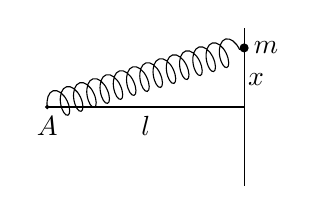
\begin{tikzpicture}
	\draw (0.5,0) node [below] {$A$} -- (3,0) node [midway, below] {$l$} (3,-1) -- (3,1);
	\draw [snake=coil, segment amplitude=5pt, segment length=5pt] (0.5,0) -- (3, 0.75);
	\draw [fill] (3, 0.75) circle (0.05) node [right] {$m$};
	\draw [fill] (0.5, 0) circle (0.02);
	\node at (3.15,0.35) {$x$};
\end{tikzpicture}
\end{document}